In the dominant optical framework of the 18th century, light was conceived as a stream of discrete particles governed by Newtonian mechanics. Isaac Newton’s \textit{Opticks} (1704) formalized this corpuscular model, arguing that light rays consist of minute corpuscles emitted from luminous bodies and traveling in straight lines. Reflection was explained as an elastic rebound from surfaces, while refraction was attributed to short-range attractive forces exerted by denser media, accelerating the particles and bending their trajectories toward the normal. This mechanism allowed Newton to derive Snell’s law within a particle-based system, predicting path changes through momentum conservation and force asymmetries at material boundaries.

To support the theory, Newton conducted a series of controlled experiments using prisms, lenses, and narrow apertures. He systematically investigated the behavior of light under dispersion, interference, and filtering conditions, recording the colors and intensities projected onto screens. In his most influential experiment, he demonstrated that white light could be decomposed into component colors using a glass prism and then recombined into white light using a second prism positioned in reverse. This suggested to him that color was not a modification of light by the prism but rather an intrinsic property of the individual corpuscles comprising each spectral component.

The corpuscular model accounted for key optical observations such as rectilinear propagation, sharp-edged shadows, and well-defined reflections from mirrors. It also offered an appealing theoretical coherence: by avoiding dependence on any physical transmission medium, the theory preserved the principle of action at a distance and aligned with Newton’s general program of universal mechanics. The absence of wave-like spreading or medium drag reinforced the view that light moved through empty space according to the same deterministic principles that governed celestial and terrestrial bodies.

A competing model had been introduced by Christiaan Huygens in 1678, proposing that light propagated not as a stream of particles but as a continuous wave. In this formulation, each point on a wavefront was treated as a source of secondary spherical disturbances, which spread outward in all directions. The superposition of these wavelets formed a new wavefront — defined as the envelope tangent to all secondary spheres — a geometric construction now known as the Huygens principle. This approach permitted derivation of the laws of reflection and refraction using purely geometric reasoning and offered an alternative to the ballistic model without invoking interfacial forces.

Huygens’ wave theory reproduced Snell’s law by modeling light as a wavefront that changes orientation when passing into a medium where wave speed decreases. This accounted for refraction by assigning slower propagation to denser materials, a reversal of the corpuscular model’s velocity assumption, later confirmed experimentally. The wave approach also gave qualitative explanations for diffraction and interference, though these effects had not yet been studied in systematic detail.

The theory required a universal propagation medium, the luminiferous ether, assumed to carry transverse vibrations through empty space. This posed internal difficulties: the ether needed to be rigid enough for high wave speeds but remained undetectable in mechanical or optical measurements. The model also offered no obvious account for sharply defined edges or specular reflection, which limited its compatibility with geometric optical effects.

By the early 1800s, the corpuscular theory retained institutional dominance in British science. Newton’s \textit{Opticks}, first published in 1704 and reissued in expanded editions through the mid-18th century, remained the authoritative source on optical behavior. Its treatments of reflection, refraction, and chromatic dispersion were widely accepted as definitive, and its success in reproducing geometric light paths reinforced its credibility within Newtonian mechanics.

On the continent, especially within the French Academy of Sciences, Huygens’ wave theory received more sustained attention, though it remained a minority position. Even as late as 1815, standard French accounts described diffraction as a peripheral anomaly rather than a core optical effect. Classical phenomena — mirror reflection, Snell’s law, and prism-induced color separation — were consistent with both frameworks. In the absence of distinct, falsifiable predictions, theoretical preferences were often shaped by broader methodological and philosophical alignments.

In 1801, Thomas Young presented experiments to the Royal Society showing that monochromatic light passing through two narrow, parallel slits produced a regular pattern of alternating bright and dark fringes on a distant screen. The results depended sensitively on slit geometry and wavelength, and the visibility of the fringes required careful alignment. The interference pattern was stable, reproducible, and inconsistent with the additive behavior of independent particles traveling in straight lines.

Young explained the pattern using the principle of superposition: coherent wavefronts emanating from the two slits combined with relative phase shifts that depended on path difference. At some locations, the waves interfered constructively; at others, destructively. While this interpretation was met with skepticism in Britain, where Newtonian mechanics held institutional authority, it found more interest in France. There, analytic approaches to physical phenomena were gaining prominence, and interference was increasingly viewed as a direct signature of wave behavior.

In the 19th century, the French Academy of Sciences organized public prize competitions to address unresolved scientific questions. These Grand Prix offered formal recognition and were intended to establish clarity on foundational issues. In 1816, the Academy awarded prizes to Augustin-Louis Cauchy for his work on wave motion and to Sophie Germain for her treatment of elastic surfaces. In 1887, Henri Poincaré received a prize for his submission on the n-body problem in celestial mechanics, which introduced new methods in dynamical analysis. The competitions were used to identify mathematically rigorous approaches and to elevate theories that could produce reliable predictions.

In 1818, the Academy announced a prize for the best theoretical account of diffraction. At the time, no existing model could give a complete explanation of the observed phenomena. The corpuscular theory remained standard in Britain, while some continental physicists were exploring wave-based descriptions grounded in interference. The competition was intended to evaluate which approach could produce quantitatively accurate results and remain consistent with experimental data.

Only two entries were received. The first, now lost and submitted anonymously, was rejected outright. The committee noted its neglect of known experimental results, its unfamiliarity with prior work by Young and Fresnel, and its numerous conceptual and computational errors. The second submission, authored by Augustin-Jean Fresnel, presented a detailed mathematical treatment of diffraction using the wave hypothesis. Fresnel extended Huygens’ geometric principle by modeling light as a scalar disturbance with definable amplitude and phase. He introduced an integral formulation in which secondary wavelets emanating from every point on a wavefront interfered according to phase delay, yielding precise intensity predictions behind apertures and opaque obstacles — derived entirely from geometry and propagation delay, without recourse to forces or ballistic mechanisms.

The response from the judging committee exposed a deep divide. Siméon Denis Poisson, an influential Newtonian, examined Fresnel’s equations with the aim of identifying contradictions. He derived what he considered a decisive counterexample: if the wave theory were valid, then a circular opaque disk should produce a bright spot at the center of its geometric shadow. From the perspective of corpuscular optics, such a prediction was absurd. That region received no direct rays and should remain dark. Poisson concluded that this result — clearly at odds with particle reasoning — invalidated Fresnel’s model as a whole.

Dominique Arago, also on the committee but less ideologically aligned with Newtonian mechanics, recognized that Poisson’s objection could be tested directly. He constructed an experimental apparatus using a monochromatic point source, a small circular obstruction, and a screen positioned along a collimated beam path. Under proper alignment, a narrow bright point consistently appeared at the center of the shadow — exactly as predicted by Fresnel’s analysis. The result was repeatable, insensitive to minor perturbations, and could not be reconciled with any particle-based mechanism. It provided direct empirical confirmation that phase-based wave interference governed the observed pattern.

The confirmation of the Arago spot did more than resolve a challenge to the wave theory. It introduced a new standard for evaluating physical theories: the ability to produce precise, testable predictions from mathematical formulations applied to specific boundary conditions. Fresnel’s analysis predicted a bright point at the center of a circular shadow — a result that followed directly from the wave model but seemed implausible to advocates of the corpuscular view.

The corpuscular theory could not reproduce the observed intensity maximum. No assumption about particle trajectories, angular spread, or probabilistic scattering could account for constructive illumination at the shadow’s center. The appearance of the Arago spot showed that physical models must be judged by whether their equations generate correct spatial distributions, not by whether their assumptions align with intuition. Predictive precision replaced interpretive plausibility as the standard for theoretical acceptance.

\begin{figure}[h]
\centering
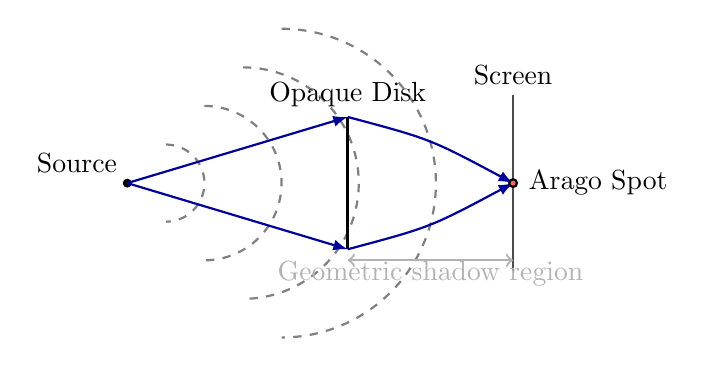
\begin{tikzpicture}[scale=0.7, thick]

% Styles
\tikzstyle{wavefront}=[gray, dashed]
\tikzstyle{lightpath}=[->, >=latex, blue!60!black]
\tikzstyle{obstacle}=[line width=1.2pt]
\tikzstyle{screen}=[line width=1pt, gray!60!black]
\tikzstyle{spot}=[fill=red!60, draw=black]

% Point source
\filldraw[black] (-4,0) circle (0.06) node[above left] {Source};

% Wavefronts (concentric arcs)
\foreach \r in {0.7,1.4,2.1,2.8}
    \draw[wavefront] (-4,0) ++(\r, \r) arc[start angle=90, end angle=-90, radius=\r];

% Opaque disk (cross-section as vertical bar)
\draw[obstacle] (0,-1.2) -- (0,1.2);
\node[above] at (0,1.2) {Opaque Disk};

% Light paths diffracted around disk to spot
\draw[lightpath] (-4,0) -- (0,1.2);
\draw[lightpath] (-4,0) -- (0,-1.2);
\draw[lightpath] (0,1.2) .. controls (1.5,0.8) .. (3,0);
\draw[lightpath] (0,-1.2) .. controls (1.5,-0.8) .. (3,0);

% Screen
\draw[screen] (3,-1.6) -- (3,1.6);
\node[above] at (3,1.6) {Screen};

% Arago spot
\filldraw[spot] (3,0) circle (0.07);
\node[right] at (3.1,0) {Arago Spot};

% Shadow label
\draw[gray!60, <->] (0,-1.4) -- (3,-1.4);
\node[gray!60] at (1.5,-1.65) {Geometric shadow region};

\end{tikzpicture}
\caption{Diffraction around a circular obstacle produces constructive interference at the center of the geometric shadow — the Arago spot.}
\end{figure}

This standard was challenged again in the early 20th century, when new experiments revealed optical behavior that neither classical wave theory nor classical particle theory could explain in full. The concept of wave–particle duality arose in response to this fragmentation.

Diffraction, interference, and polarization aligned with wave theory, particularly as formulated by Maxwell’s equations, which described light as a transverse electromagnetic wave propagating through space. In contrast, the photoelectric effect and Compton scattering could not be explained by continuous fields. These phenomena exhibited discrete energy transfers and momentum conservation consistent with particle-like interactions. Each domain appeared to demand a separate formalism: wave optics for propagation, and quantum mechanics for emission and absorption.

This division extended into mathematical treatment. Wave behavior was modeled using Maxwell’s classical field equations, which predicted interference patterns and polarization with high accuracy. Particle behavior was captured by early quantum mechanics, where photons were treated as quantized packets of energy and momentum. No unified equation described both regimes. As a result, physicists adopted a pragmatic view: light exhibits wave-like properties in some experiments and particle-like behavior in others. The term “duality” entered usage as a placeholder for the absence of a single consistent framework. Though heuristically useful, this terminology preserved the conceptual split rather than resolving it.

Quantum electrodynamics models light as a quantized electromagnetic field. Photons are defined as discrete energy–momentum quanta, arising from specific modes of the field. They are not particles following trajectories, nor are they oscillations in a medium. The field exists across spacetime and interacts with detectors in localized energy exchanges. Its behavior is governed by operator equations that encode propagation and interaction.

Photon states are described in Fock space, built from the quantized normal modes of the electromagnetic field. Each state is labeled by momentum, polarization, and frequency. Measurements are represented by projection operators, and outcomes correspond to specific detector responses. The theory provides exact rules for calculating detection probabilities, scattering amplitudes, and energy transfers without relying on classical analogies.

The Arago spot results from coherent superposition of field amplitudes originating from different spatial regions. Each amplitude accumulates a phase determined by its path and boundary interactions. The total intensity is computed by summing complex amplitudes and taking the modulus squared. This produces the observed distribution on a screen, including a central bright point where contributions interfere constructively.

When the light intensity is reduced to the single-photon level, individual detection events remain pointlike. Over time, the same interference pattern emerges from their distribution. This confirms that the probability amplitudes are governed by phase coherence even when the field is quantized. The spot does not depend on ensemble behavior but on the linearity of the field equations and the phase relationships between contributing paths.

The equations of quantum electrodynamics predict the observed intensity pattern without invoking wave–particle duality. All observable results come from the field equations, boundary conditions, and measurement rules. The appearance of the Arago spot reflects the calculated distribution of detection probabilities. No additional interpretive model is needed beyond what the field theory already supplies.

\begin{SideNotePage}{
  \textbf{Model Comparison:} \par Three theoretical models are applied to two classic experiments: the double slit and the photoelectric effect. The goal is to highlight where predictions agree with experiment and where they fail.

  \vspace{1.5em}
  \textbf{Top (Corpuscular):} \par Double-slit: no interference, \( I(x) \sim e^{-(x - x_1)^2} + e^{-(x - x_2)^2} \). \par Photoelectric: emission occurs only if photon energy exceeds the threshold, \( R \sim \Theta(\omega - \phi) \).

  \vspace{1.5em}
  \textbf{Middle (Wave):} \par Double-slit: interference arises from wave superposition, \( I(x) \sim \cos^2(x) \). \par Photoelectric: continuous energy absorption incorrectly predicts emission at all \( \omega \), \( R \sim 1 \).

  \vspace{1.5em}
  \textbf{Bottom (QED):} \par Double-slit: coherent paths interfere, \( I(x) \sim |\Psi_1 + \Psi_2|^2 \sim \cos^2(x) \). \par Photoelectric: decoherent transition amplitudes yield \( R \sim |\mathcal{M}|^2 \sim \Theta(\omega - \phi) \). The same path integral formalism applies, but coherence conditions differ.

  \vspace{1.5em}
  Green frames highlight where predictions match experimental outcomes.
}{13_PoissonsSpot/6135-.pdf}
\end{SideNotePage}
